\section{Background} \label{section_background}

%The \scps respond to a function of temperature. To precisely control this complicated actuator, an electrical microprocessor was used. Therefore, the methods for electrically operating \scps and investigating their characteristics are discussed.

\scps - otherwise called as Baughman muscles or Haines muscles - are new-generation actuator which were announced in 2014.
%What makes the \scps special is its large strain and its work density that is only exceeded by shape-memory alloys.
Since these artificial muscles are thermally actuated, previous researches had established an appropriate method for heating the muscles.
In this section, methods for fabricating, actuating, and cooling \scps are introduced.
Also, principle of antagonism was described, which was utilized for making an \antanospace.

\subsection{SCP Artificial Muscles}
The \scps used in this paper were made by twisting silver-painted nylon thread (Conductive Sewing Thread Size 92, Shieldex), which was found to be the best in terms of strain and force production \cite{haines}. First, the conductive thread was piled up four times to make its length be \SI{50}{\centi\meter}. Each side of thread was connected to washers. Then, a wire was hung to one of the washer and a motor to the other. (Figure \ref{silverSCP_2})
As illustrated in figure \ref{silverSCP_illust}, the motor was rotated until the thread created a coil \cite{fab_coil}. After making same one again, two coils were overlapped to each other, making stable form. 
Lastly, they were heated up under an electric current.\footnote{\SI{2.5}{\ampere} was applied and stopped when smoke occurred. While repeating heating and cooling about ten times, the length at ambient temperature got longer and reached at a constant length.} By using this method, \scp was made, which is \SI{10}{\centi\meter} - \SI{11}{\centi\meter} in length and \SI{2.5}{\ohm} in electric resistance($ R $) at ambient temperature with no external force.



\begin{figure}[b]
	\centering
	\begin{subfigure}{.22\linewidth}
		\centering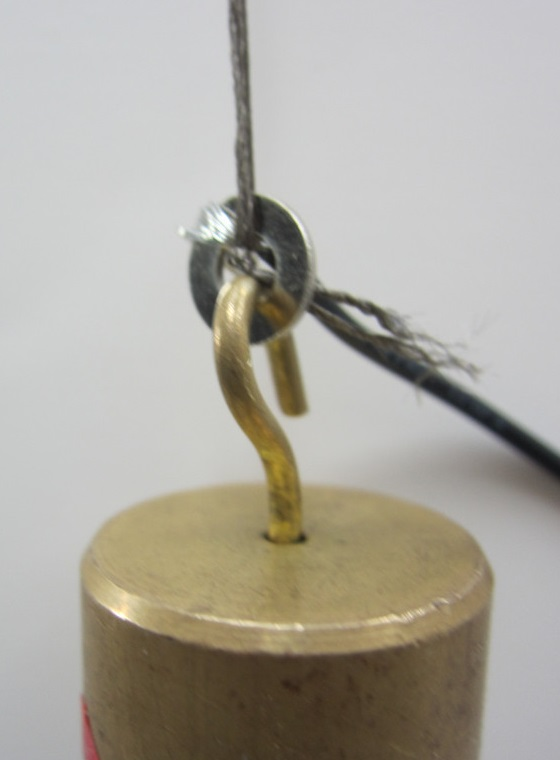
\includegraphics[width=\textwidth]{small_silverSCP_3_v2.jpg}
		\caption{\label{silverSCP_2}}
	\end{subfigure}
	~
	\begin{subfigure}{.57\linewidth}
		\centering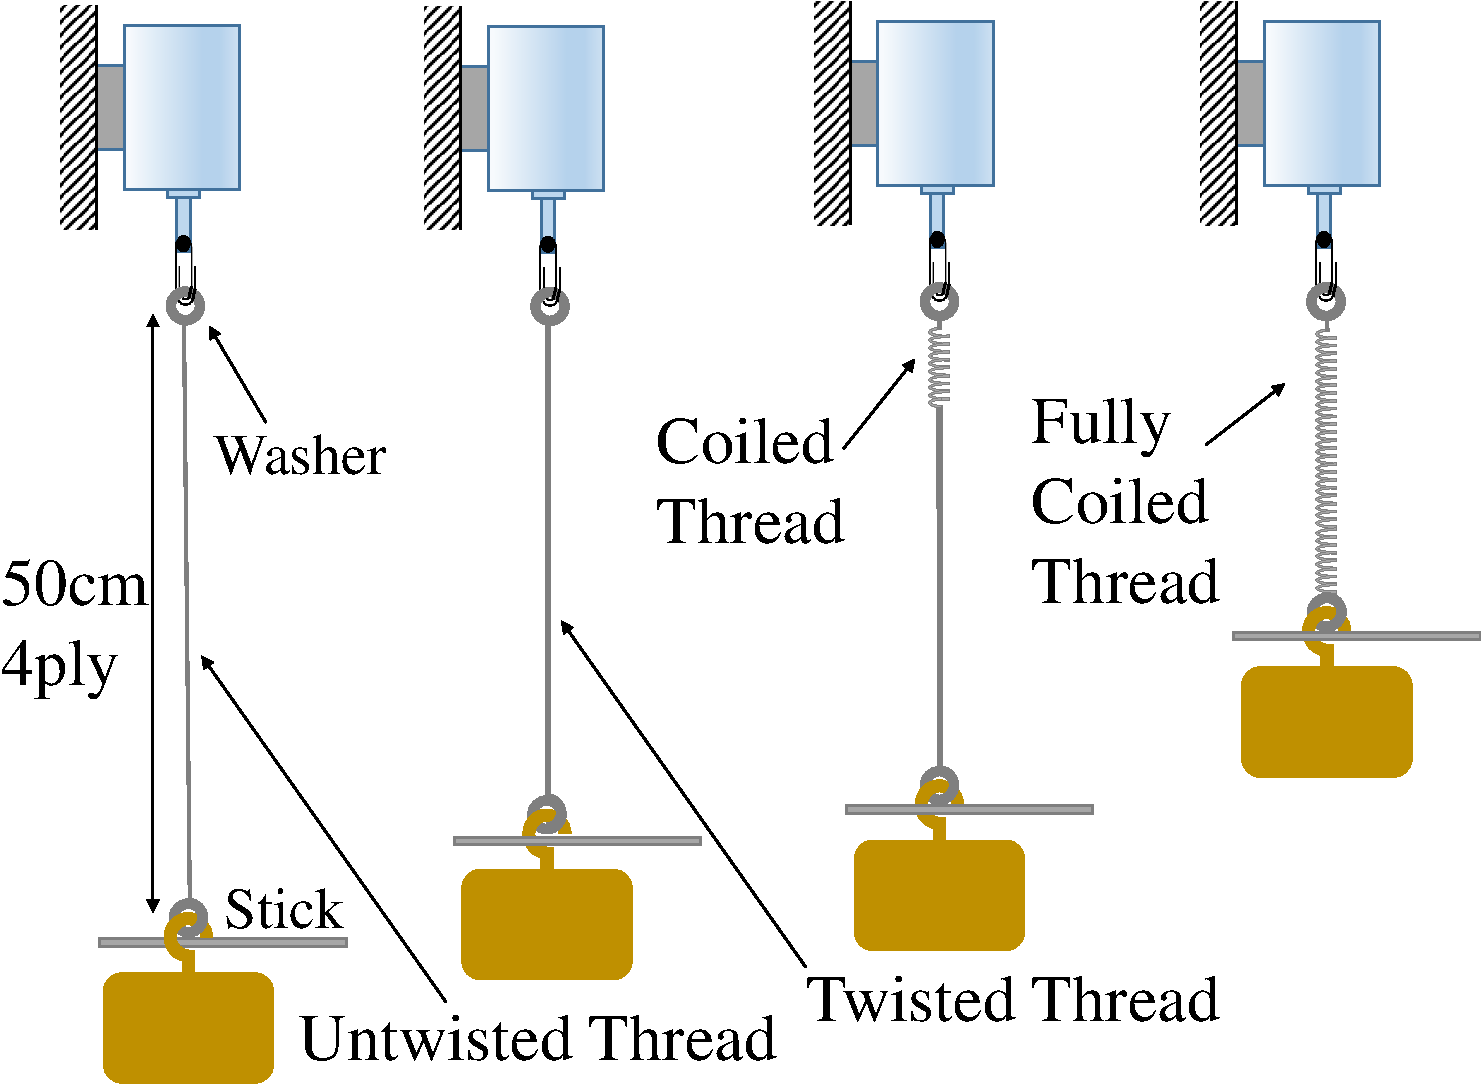
\includegraphics[width=\textwidth]{Fab_illust_v2_crop.pdf}
		\caption{\label{silverSCP_illust}}
	\end{subfigure}
	~
	\begin{subfigure}{.15\linewidth}
		\centering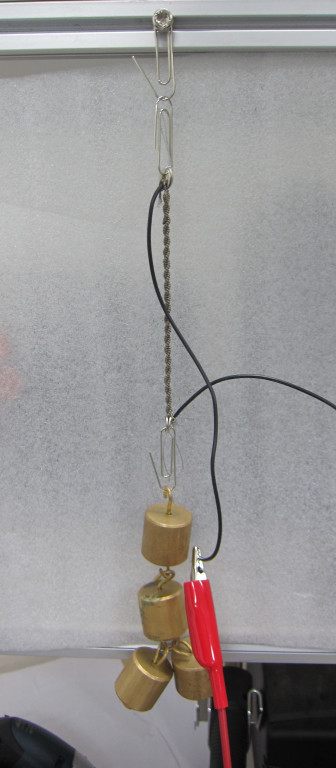
\includegraphics[width=\textwidth]{small_silverSCP_7.jpg}
		\caption{\label{silverSCP_annealing}}
	\end{subfigure}
	\caption[Process of making \scps with silver-painted nylon thread]{\subref{silverSCP_2} 4-ply, \SI{50}{\centi\meter} thread bundle's each side was attached to washers. The upper end was hung on motor, and the lower end was attached to \SI{400}{\gram} weight with a wire inserted in between washer and thread. \subref{silverSCP_illust} To twist a thread until it created a coil, the bottom was fixed with a stick. Then, two super coiled polymers were made. Their upper parts were attached to one clip and their lower parts were hung on \SI{400}{\gram} weight. Coiled thread's thickness is exaggerated in this figure. \subref{silverSCP_annealing} By these processes, the \scpnospace, which has wire on its each side, was made. Finally, they were annealed until their length at ambient temperature didn't get longer.}
	\label{silverSCP_makingof}
\end{figure}

%\subsection{Actuation of the SCP Artificial Muscles} \label{subsection_actuation}
%As discussed in the previous section, the \scp was made with conductive thread in order to electrically control the heat speed. The electrical resistance of the \scp was $R=\SI{2.5}{\ohm}$, so the power $P$ was supplied by applying voltage $V=\sqrt{PR}$. The voltage was controlled by MOSFET and PWM generation of Arduino Uno.

%\subsection{Forced Air Cooling of the SCP Artificial Muscles}\label{section_electrical_control}

Since these \scps have electrical conductivity, they were thermally actuated by Joule heat caused by voltage.
Power $ P $ was applied to the muscles by controlling the voltage as $ V=\sqrt{PR} $, by using MOSFET and PWM generation of Arduino Uno.

On the other hand, in terms of cooling artificial muscles, water and forced air are considered to be a natural method in operating temperature \cite{madden}.
%Even if \scp can be naturally cooled, but natural cooling speed isn't fast enough.
In Wu \etal, cold water reservoir was used to implement fast finger movements \cite{finger}.
But, water cooling is not appropriate for electrically conductive \scpsnospace. Accordingly, forced air cooling was utilized by using compressed air can.
Muscles was surrounded by cylindric tube to make the air directly flow through the muscles.
This tube was made by thin, plastic tube to minimize the effect on specific heat of the muscles.


\subsection{Principle of Antagonism} \label{subsection_anta}
\scps can be easily heated by applying the electric current. However, cooling demands more sophisticated procedure. Also, muscles can produce force only by contracting, not by relaxing. This means that \scps can't be directly applied to robots which have to produce force in various positions.
Therefore, principle of antagonism was used, which is known to be energy-optimal for various tasks and its joints be intrinsically flexible \cite{antagonism}. 
Additionally, we could get the same effect as cooling one muscle by heating another one, since two of the muscles contracts complementarily.
This principle was utilized for making \antanospace, which will be described in section \ref{section_appa}.

\begin{figure}[b]
	\centering
	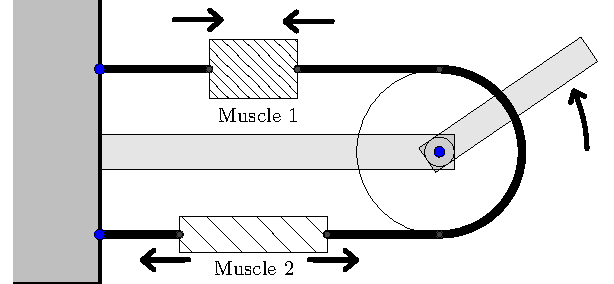
\includegraphics[width=0.8\textwidth]{AntaSchematic_v3.pdf}
	\caption[Principle of Antagonism.]{Principle of antagonism. If one of the muscles contracts, then the other elongates.}
	\label{antagonism}
\end{figure}


